\pgfsetplotmarksize{0pt}
\begin{figure}
 \centering
 \caption{\label{fl_conv7}UflLib/Euclid/1111EuclS.txt},
 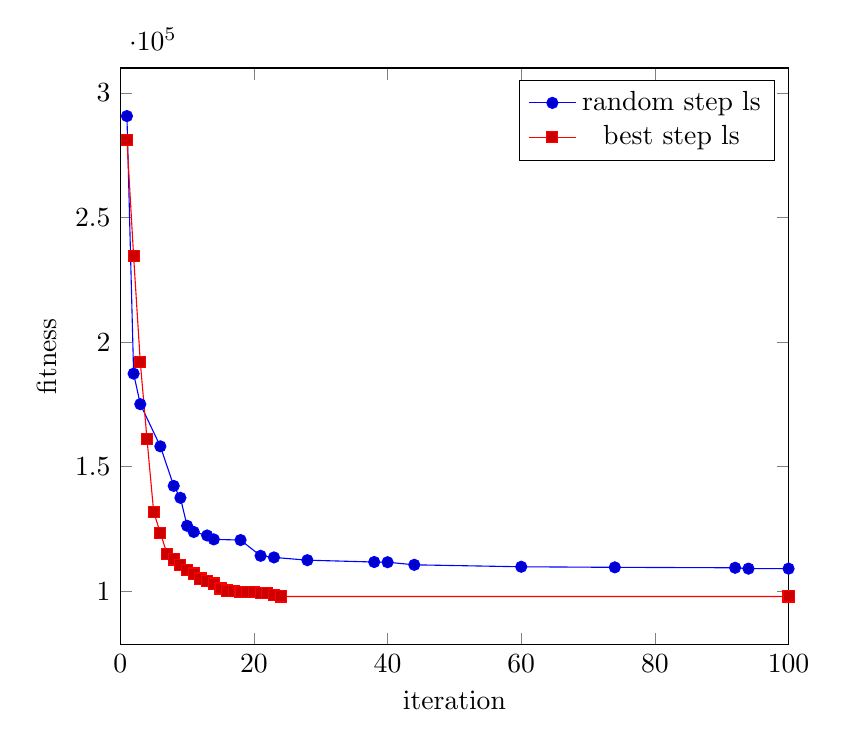
\begin{tikzpicture}
 \begin{axis}[
   width=0.7\textwidth,
   scale only axis,
   xlabel=iteration,
   ylabel=fitness,
   xmin=0,xmax=100,
   domain=0:100]
   \addplot coordinates {
     (0,inf)
     (1,290749)
     (2,187336)
     (3,175080)
     (6,158151)
     (8,142273)
     (9,137485)
     (10,126261)
     (11,123770)
     (13,122368)
     (14,120797)
     (18,120527)
     (21,114198)
     (23,113557)
     (28,112447)
     (38,111707)
     (40,111627)
     (44,110582)
     (60,109798)
     (74,109573)
     (92,109399)
     (94,109048)
     (100,109048)
   };
   \addlegendentry{random step ls}
   \addplot coordinates {
     (0,inf)
     (1,281143)
     (2,234436)
     (3,191891)
     (4,161085)
     (5,131828)
     (6,123352)
     (7,115024)
     (8,112733)
     (9,110438)
     (10,108468)
     (11,107072)
     (12,105066)
     (13,104050)
     (14,103061)
     (15,101070)
     (16,100249)
     (17,99981)
     (18,99814)
     (19,99700)
     (20,99511)
     (21,99405)
     (22,99331)
     (23,98490)
     (24,97886)
     (100,97886)
   };
   \addlegendentry{best step ls}
 \end{axis}
 \end{tikzpicture}
\end{figure}
